\section{Introduction}
\label{sec:introduction}

Many social networking, e-commerce, and web properties contain
data-derived products, which usually consist of some data mining
application exposing insights to the user. Typical products include:
``People You May Know,'' a link prediction system attempting to find
others one might know on the social
network~(c.f.~Figure~\ref{fig:pymk}); collaborative filtering, which
showcases relationships between pairs of items based on the wisdom of
the crowd~(c.f.~Figure~\ref{fig:browsemaps}); job and other entity
recommendations; and more. \linkedin\footnote{Anonymized name} is a
top-5 social network with more than 120~million members consisting of
these and twenty other data-derived products. 

The commoditization of batch computing infrastructure like Hadoop and
the rise of machine learning at Internet companies leads to complex
algorithms that run over large data sets as a core production use
case. The challenge with these products is that they must surface
hundreds of results for each of our 120~million members using
expensive link prediction or nearest-neighbor algorithms. For example,
the ``People You May Know'' system churns on more than 100~TB of data
daily to make its predictions.

Importantly, due to the dynamic nature of the social graph, this
derived data changes extremely frequently---requiring an almost
complete refresh of the data, all the while still serving existing
traffic with minimal additional latency. 

The product data cycle in this context consists of a continuous cycle
of three phases: data collection, processing and finally serving. The
data collection phase usually involves log ingestion, while the
processing phase is a distributed parallel computing infrastructure.
Interestingly, the nature of this cycle means live updates are not
necessary and nevertheless are difficult to handle, and that a batch
update should complete quickly to engender frequent pushes.
 
\begin{figure}
\centering
\subfloat[][]{\label{fig:pymk}

\includegraphics[scale=0.5]{images/pymk}
}

\subfloat[][]{\label{fig:browsemaps}
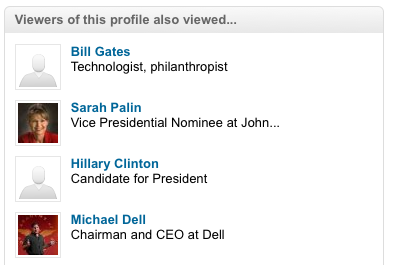
\includegraphics[width=0.9\columnwidth]{images/browsemaps}
}

\caption{\subref{fig:pymk}~The ``People You May Know'' module
\subref{fig:browsemaps}~An example collaborative filtering
application.}
\end{figure}

This paper presents read-only extensions to Project \projectname{},
our key-value solution for the final serving phase of this cycle, and
discusses how it fits into our product ecosystem. \projectname{} is
inspired by Dynamo~\cite{dynamo} and was initially designed to only
support the fast online read/write load, but its extensible storage
layer allowed us to quickly build our own custom read-only storage
engine to integrate with the offline data cycle and support these
batch-oriented use cases. At \linkedin, this system has been running
for over 2~years with our largest cluster loading around 3~TB of new
data to the site every day. 

As part of this lifecycle, we have access to an elastic pool of batch
computing infrastructure with little to no latency requirements, which
\projectname{} leverages to build its index and data files in Hadoop
to support a high throughput for batch refreshes. The system provides
excellent live serving performance: our evaluation, and the results we
see in production, show that the system yields sub-20~ms average read
times---even during data refreshes. 

\projectname{} supports instantaneous rollback, where data can be
restored to a clean copy minimizing the time in error, which helps
support fast, iterative development, especially necessary for new
feature improvements. The system also provides the ability to grow
horizontally with its ability to rebalance existing data to new nodes
without down-time. 

The key contributions of this work are:
\begin{compactitem}
\item A scalable offline index construction data pipeline 
\item Custom storage engine which leverages the operating system's
caching for cache management
\end{compactitem}

% vim: set ft=tex:
